\documentclass{article}
\usepackage[utf8]{inputenc}    % For UTF-8 character encoding
\usepackage[T1]{fontenc}       % For proper font encoding
\usepackage{lmodern}           % Improved font rendering
\usepackage{amsmath}   % For advanced mathematical formatting
\usepackage{amssymb}   % For mathematical symbols
\usepackage{geometry}  % Adjust page margins
\usepackage{enumerate} % For custom lists
\usepackage{xcolor}  % for coloring
\usepackage{amsthm}
\usepackage{pdfpages}
\newtheorem{theorem}{Theorem}[section]
\newtheorem{lemma}[theorem]{Lemma}
\newtheorem{corollary}[theorem]{Corollary}
\newtheorem{definition}[theorem]{Definition}
\usepackage{listings}  % for code listings

\lstset{frame=tb,
  language=C,
  aboveskip=3mm,
  belowskip=3mm,
  showstringspaces=false,   
  columns=flexible,
  basicstyle={\small\ttfamily},
  numbers=none,
  numberstyle=\tiny\color{gray},
  keywordstyle=\color{blue},
  commentstyle=\color{brown},
  stringstyle=\color{orange},
  breaklines=true,
  breakatwhitespace=true,
  tabsize=3
}
\geometry{top=1in, bottom=1in, left=1in, right=1in}

\begin{document}

\title{}
\author{Wang Xiyu}
\date{}
\maketitle
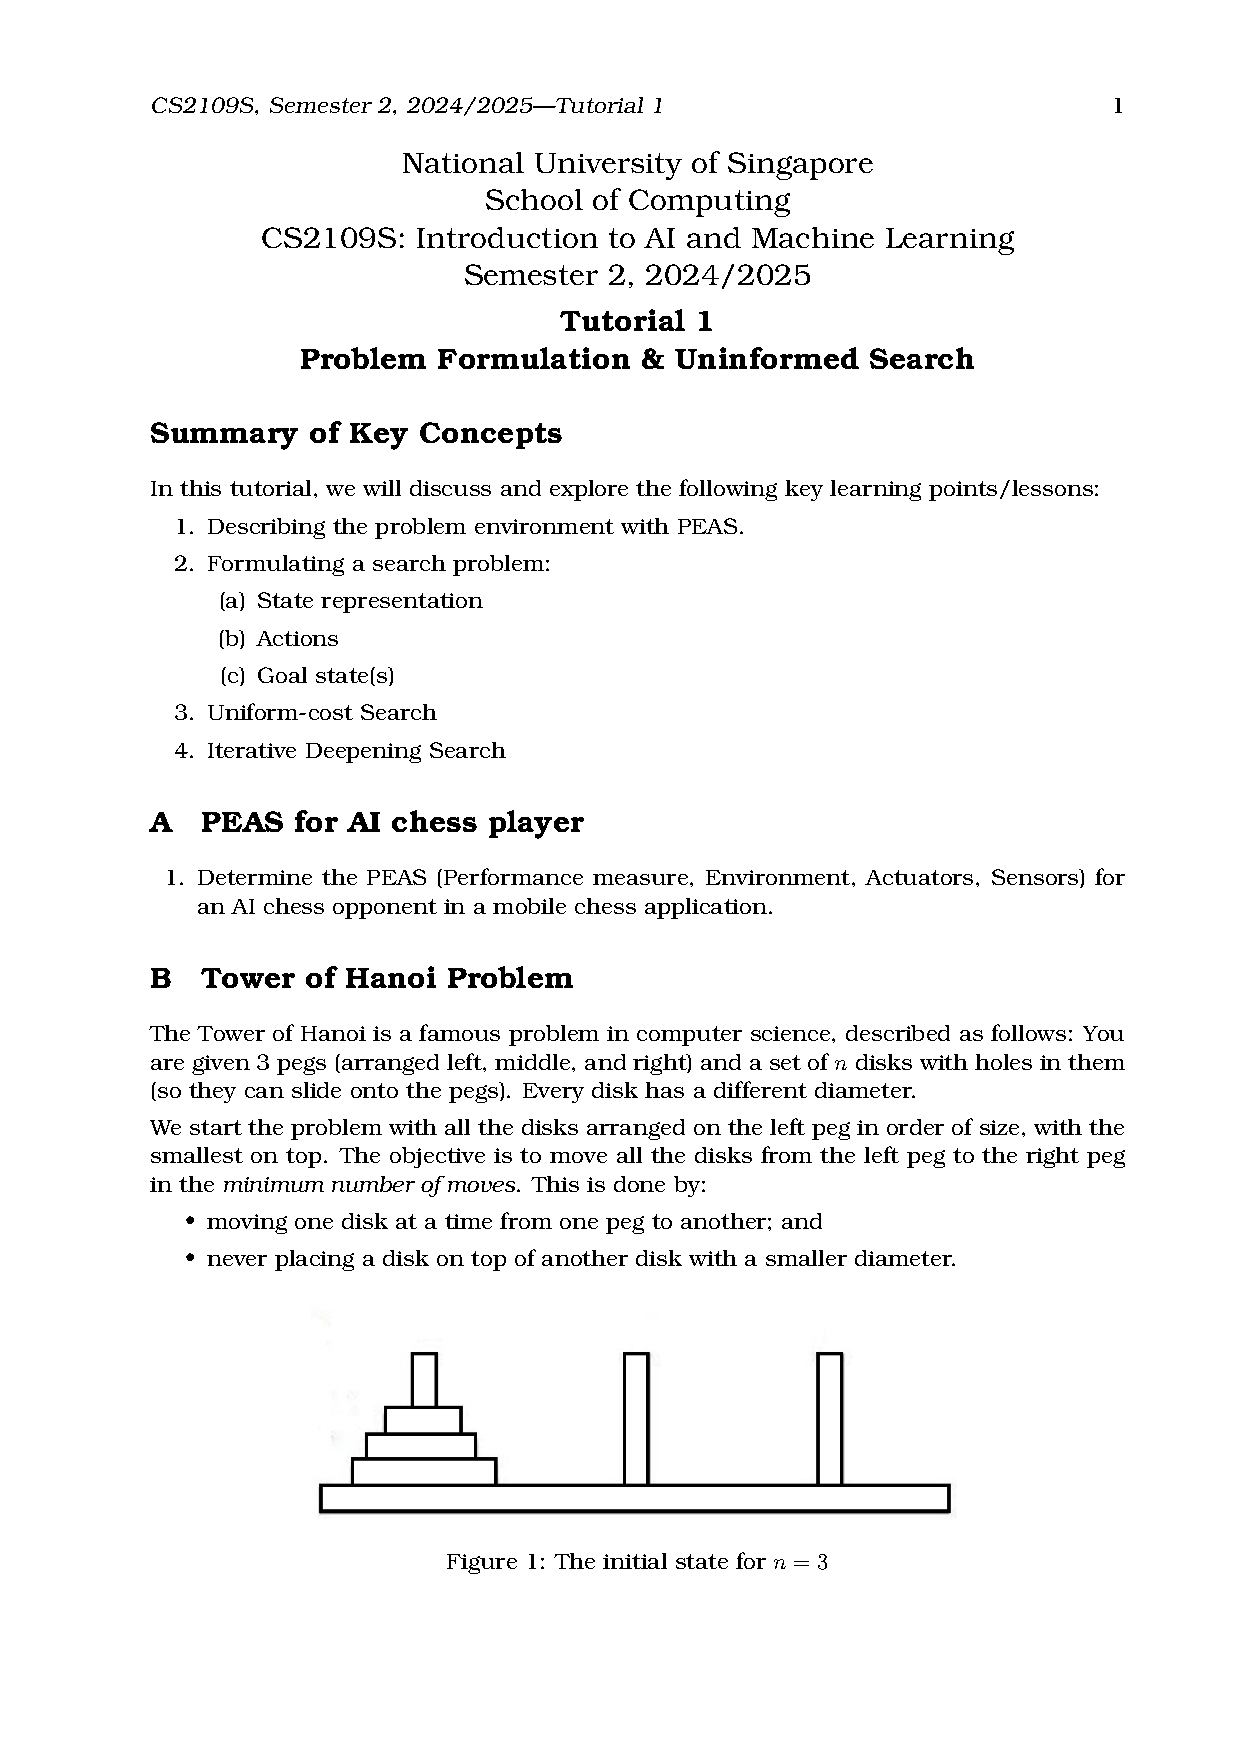
\includepdf[pages=1]{Tutorial1.pdf}
\section{1}
\subsection{}
\subsubsection*{a}
States: every possible placement scheme of all disks on all poles, represented by a tuple of lists or stacks in the form of \{[1, 2, 3, 4, 5], [], []\} etc.\newline
Initial State: the starting placement of all disks\newline
Goal States: The designated way of placing the all disks\newline
\textcolor{red} {Use set to make \{1, 2\} and \{2, 1\} to be the same state and the later is not a valid state}\newline
action: if $state_a$ can be transformed into $state_b$ my moving one disk, $state_b$ is reacheable from $state_a$ in cost 1 
\subsubsection*{Total number of states}
Loose bound:\newline
Flatten the list tuple, an action can be seen as a swap between 2 elements in the flattened list. the flattened list can then be partitioned into 3 partitions, by placing 2 separaters, the total number of arranging all disks on all 3 poles is:
\[\binom{n + 2}{2}!\]
Tighter bound after considering constraints: \newline
for each state, there are only 3 legal moves. Given state a, 
\[S = \{[d_1, d_2,\dots, d_{a-1}], [d_a, d_{a+1},\dots, d_{b-1}], [d_b, d_{b+1}, \dots d_n]\} \text{(Consider all disks are ordered)}\]
only the top of any peg can be placed onto another peg's top. Since all disks are comparable, the tops of all pegs are also comparable. WLOG
\[d_1 < d_a < d_b\]
$\forall S \in \{\text{possible arrangment }\} \exists $ exactly 3 valid movements: 
\[move(S, d_1, 1) = \{[d_2,\dots, d_{a-1}], [d_1, d_a, d_{a+1},\dots, d_{b-1}], [d_b, d_{b+1}, \dots d_n]\}\]
\[move(S, d_1, 2) = \{[d_2,\dots, d_{a-1}], [d_a, d_{a+1},\dots, d_{b-1}], [d_1, d_b, d_{b+1}, \dots d_n]\}\]
\[move(S, d_a, 2) = \{[d_1, d_2,\dots, d_{a-1}], [d_{a+1},\dots, d_{b-1}], [d_a, d_b, d_{b+1}, \dots d_n]\}\]
Therefore for in total $n$ disks, there are $3^n$ valid states. 
\subsubsection*{b}
Representation invariant: No larger disk on smaller disks in all possible states. In list tuple representation, all lists are sorted; In set tuple represented there is no need to sort since permutations are regarded as the same.
\subsection{}
Depth-Limit Search(using DFS). 
\subsection{}
$k - 1$. as there will be more choices of action from one state to another.
\includepdf[pages=2]{Tutorial1.pdf}
\section*{}

\includepdf[pages=3]{Tutorial1.pdf}
\section*{}

\includepdf[pages=4]{Tutorial1.pdf}
\section*{D}
\subsection{}
Linear search, or a tree search with braching factor 1, iterative deepening search perform in worse case scenario costs $O(n^2)$
while dfs costs $O(n)$

\subsection{}
1. In linear search there is no need to keep tracking visited as node will not be visited again whatsoever, thus search without visited memory can save up to O(n) space. For example, search in a linked list.\newline
\textcolor{red} {}
2. Search on an ordered tree, the search does not need to exhaustively explore nodes thus there is no need to keep track of visited node, saving up to O(n) space. For example, search in a ordered binary tree. \newline
\textcolor{red} {}

\end{document}
